Установим некоторые вспомогательные формулы, нужные для представления решений краевых задач в интегральной форме. Пусть
\[
	L[u] = \derps{u}{x}{y} + a(x, y) \derp{u}{x}{} + b(x, y) \derp{u}{y}{} + c(x, y) u 
\]
-- линейный дифференциальный оператор, соответствующий уравнению гиперболического типа.\\
Характеристиками уравнения являются $y = C_1$ и $x = C_2$.
Начальные условия будем задавать на кривой $y = g(x)\quad (x = \eta(y))$.

\begin{wrapfigure}[0]{r}{0.35\textwidth}
	\centering
	\includegraphics[width=0.2\textwidth]{fighyperriman.pdf}
\end{wrapfigure}
\begin{minipage}[t]{0.7\textwidth}
\begin{align*}
	&u|_{y = g} = g(x)\\
	&\left.\derp{u}{y}{}\right| =  \psi(x)
\end{align*}
\begin{align*}
	&L[u] =  \derps{u}{x}{y} + a(x, y) \derp{u}{x}{} + b(x, y) \derp{u}{y}{} + c(x, y) u \\
	&L^*[v] = \derps{v}{x}{y} - \derp{}{x}{} \left(a v \right) - \derp{}{y}{} \left(b v \right) + c  v\\
\end{align*}
\end{minipage}\\


\begin{multline*}
	vL[u] - u L^*[v] = v \derps{u}{x}{y} - u \derps{v}{x}{y} + a v \derp{u}{x}{}  + u \derp{}{x}{} \left(a v \right) + b v \derp{u}{y}{} + u \left(b v \right) =\\
	= \frac{1}{2} \derp{}{x}{} \left(v \derp{u}{y}{} \right) - \frac{1}{2} \derp{v}{x}{} \derp{u}{y}{} + \frac{1}{2} \derp{}{y}{} \left(v \derp{u}{x}{} \right) - \frac{1}{2} \derp{v}{y}{} \derp{u}{x}{} - \frac{1}{2} \derp{}{x}{} \left(u \derp{v}{y}{} \right) + \frac{1}{2} \derp{u}{x}{} \derp{v}{y}{} - \frac{1}{2} \derp{}{y}{} \left(u \derp{v}{x}{} \right) + \frac{1}{2} \derp{u}{y}{} \derp{v}{x}{} = \\
	= \frac{1}{2} \derp{}{x}{} \left(v \derp{u}{y}{} - u \derp{v}{y}{} + 2 a u v \right) + \frac{1}{2} \derp{}{y}{} \left(v \derp{u}{x}{} - u \derp{v}{x}{} + 2 b u v \right)
\end{multline*}
Пришли к \textit{дивергентному виду}.

Из этого следует, что $L^*$ -- сопряжённый оператор.

\[
	v L[u] - u L^*[v] = \frac{1}{2} \derp{}{x}{} \left( v \derp{u}{y}{} - u \derp{v}{y}{} + 2 auv \right) + \frac{1}{2} \derp{}{y}{}\left(v \derp{u}{x}{} - u \derp{v}{x}{} + 2 b u v\right)
\]
\begin{multline*}
	\iint\limits_D\left[v L[u] - u L^* [v] \right] = \frac{1}{2} \oint \left[ \left(v \derp{u}{y}{} - u \derp{v}{y}{}  + 2 au v\right)\, dy - \left(v \derp{u}{x}{} - u \derp{v}{x}{} + 2 b u v \right)\, dx \right] = \\
	= - \frac{1}{2} \int\limits_A^B \left(v \derp{u}{x}{} - u \derp{v}{x}{} + 2 buv\right)\, dx + \frac{1}{2} \int\limits_B^C \left(v \derp{u}{y}{} - u \derp{v}{y}{} + 2 auv\right)\, dy +{}\\+ \frac{1}{2} \int\limits_C^A \left[\left(v \derp{u}{y}{} - u \derp{v}{y}{} + 2 u v a\right)\, dy + \left(u \derp{v}{x}{} - v \derp{u}{x}{} + 2 b u v \right)\, dx\right] =\\
	= - \frac{1}{2} uv \Big|_A^B + \frac{1}{2} \int\limits_A^B u \left( 2 \derp{v}{x}{} - 2 bv \right)\, dx + \frac{1}{2} uv \Big|_B^C + \frac{1}{2} \int\limits_B^C u \left(-2 \derp{v}{y}{} \right)\, dy + \frac{1}{2} \int\limits_A^C \left[\ldots \right]\, dx dy
\end{multline*}
Потребуем $\derp{v}{x}{} - bv = 0 \big|_{y = Y_0}, \quad \derp{v}{y}{} - a v = 0 \big|_{x = X_0}$\\

\begin{equation}
	v = C e^{\int\limits_{x_0}^x b \,dx} \qquad v = C e^{\int\limits_{y_0}^y a \,dy}
	\label{equ:equRiman}
\end{equation}
где $C = 1$.\\
$v(x, y, x_0, y_0)$ -- \textit{функция Римана}.\\

Для функции Римана должно выполняться $v(x_0, y_0, x_0, y_0) = 1$ и она должна удовлетворять $L^*(v) = 0$. Известно, что $L[u] = f(x, y)$, тогда
\[
	vL[u] = v f(x, y)
\]
Тогда для интеграл принимает вид
\[
	\iint\limits_D v f(x, y)\, dx dy = \frac{1}{2} \left(uv\Big|_A - u v\Big|_B \right) + \frac{1}{2} \left(uv\Big|_C - uv \Big|_B \right) + \frac{1}{2} \int\limits_C^A \left[ \ldots \right]\, dx dy
\]
Для
\[
	B= (x_0, y_0) \Rightarrow v\Big|_B = 1,
\]
мы получаем
\[
	v u(B) = \frac{uv\big|_A + u v \big|_B}{2} + \frac{1}{2} \int\limits_C^A \left[\left(v \derp{u}{y}{} - u \derp{v}{y}{}  + 2 auv\right)\, dy + \left(u \derp{v}{x}{} - v \derp{u}{x}{} + 2 bu v \right)\, dx \right] - \iint\limits_D f(x,y)\, dx dy
\]
%Двойной интеграл от разности $vl[u] - u l^*[v]$ по некоторой области $g$, ограниченной кусочно-%гладким контуром $c$, равен 
%\[
%	\iint\limits_g (v l[u] - u l^*[v] )\, d\xi \, d\eta = \int\limits_c (h\, d\eta - k\, d\xi)
%\]
%где $u$ и $v$ - произвольные дважды дифференциируемые функции(двумерная формула Грина).
\newpage
\begin{example}{Телеграфное уравнение}
\[
	\derp{u}{x}{2} = LC \derp{u}{t}{2} + \left(RC + LG \right) \derp{u}{t}{} + RGu
\]
Начальные условия ($t = 0$): 
\begin{align*}
	u &= f(x);\\
	\derp{u}{t}{} &= g(x)
\end{align*}
\[
		a_0 = LC, \quad RC - LG = 2 b_0, \quad RG = C_0
\]
\[
	\derp{u}{x}{2} = a_0 \derp{u}{t}{2} + 2 b_0 \derp{u}{t}{} + C_0 u
\]
Будем искать $u$ в виде 
\[
	u = e^{- \frac{b_0}{a_0}t} \cdot w(x, t)
\]
\begin{align*}
	&\derp{u}{x}{} = e^{- \frac{b_0}{a_0}t} \derp{w}{x}{} &\derp{u}{x}{2} = e^{- \frac{b_0}{a_0}t} \derp{w}{x}{2}\\
	&\derp{u}{t}{} = - \frac{b_0}{a_0} e^{- \frac{b_0}{a_0} t} w(x,t) + e^{- \frac{b_0}{a_0}t} \derp{w}{t}{}
	&\derp{u}{t}{2} = \frac{b_0^2}{a_0^2} e^{-\frac{b_0}{a_0}} w(x, t) - 2 \frac{b_0}{a_0} \derp{w}{t}{} e^{- \frac{b_0}{a_0}t} + e^{- \frac{b_0}{a_0}} \derp{w}{t}{2}
\end{align*}

\[
	\derp{w}{x}{2} = a_0 \derp{w}{t}{2} - \cancel{2 b_0 \derp{w}{t}{}} + \cancel{\frac{b_0^2}{a_0} w} - \cancel{2} \frac{b_0^2}{a_0} w + \cancel{2 b_0 \derp{w}{t}{}} + c_0 w
\]\\
\[
	\begin{cases}
		\displaystyle\derp{w}{x}{2} = a_0 \derp{w}{t}{2} + \left(c_0 - \frac{b_0^2}{a_0} \right) w\\
		t = 0 \quad w(x, 0) = f(x) \quad \derp{w}{t}{} = g(x) + \frac{b_0}{a_0} f(x)
	\end{cases}
\]
\[	
	\derp{w}{t}{2} = \underbrace{\frac{1}{a_0}}_{a^2} \derp{w}{x}{2} + \underbrace{\frac{b_0 - a_0 c_0}{a_0^2}}_{b^2} w
\]
Итак
\[
	\begin{cases}
		\displaystyle\derp{w}{x}{2} = a^2 \derp{w}{t}{2} +b^2 w\\
		t = 0 \quad w(x, 0) = f(x) \quad \derp{w}{t}{} = g(x) + \frac{b_0}{a_0} f(x)
	\end{cases}
\]\\

Вернёмся к характеристическим переменным:
\[
	\begin{cases}
		\xi = \frac{b}{a}(x + at)\\
		\eta = \frac{b}{a}(x - at)
	\end{cases}
	\qquad
	\begin{cases}
		t = \frac{\xi - \eta}{2b}\\
		x = \frac{(\xi + \eta)}{2}\frac{a}{b}
	\end{cases}
\]
тогда 
\begin{align*}
	&\derp{w}{t}{} = \left(\derp{w}{\xi}{} - \derp{w}{\eta}{} \right)b &\derp{w}{t}{2} = b^2 \left(\derp{w}{\xi}{2} - 2 \derps{w}{\xi}{\eta} + \derp{w}{\eta}{2} \right)\\
	&\derp{w}{t}{} = \frac{b}{a} \left(\derp{w}{\xi}{}  + \derp{w}{\eta}{}\right)
	&\derp{w}{x}{2} = \frac{b^2}{a^2} \left(\derp{w}{\xi}{2} + 2 \derps{w}{\xi}{\eta} + \derp{w}{\eta}{2} \right)
\end{align*}
В итоге
\[
	4 b^2 \derps{w}{\xi}{\eta} + b^2 w = 0
\]
Следовательно
\[
	\derps{w}{\xi}{\eta} = - \frac{w}{4}
\]
\end{example}

\begin{example}{Решение линейного уравнения гиперболического типа}
Найдём решение линейного уравнения гиперболического типа
\[
	\derps{w}{\xi}{\eta} + \frac{1}{4}w = 0
\]
удовлетворяющее начальным условиям на кривой $S$ ($t = 0$),
\begin{gather*}
	\xi = \eta \quad x = \frac{a}{b} \xi \quad w = f\left(\frac{a}{b} \xi\right)\\
	\derp{w}{\xi}{} - \derp{w}{\eta}{} = g\left(\frac{a}{b}\xi\right) + \frac{b_0}{a_0} f\left(\frac{a}{b} \xi\right)
\end{gather*}
\[	
	L[w] = \derps{w}{\xi}{\eta} + \frac{w}{4} \qquad L^*[v] = L[v] = \derps{w}{\xi}{\eta} + \frac{v}{4}
\]

\begin{multline*}
	v L[w] - w L[v] = v \derps{w}{\xi}{\eta} - w \derps{w}{\xi}{\eta} = \\ = \frac{1}{2} \derp{}{\xi}{} \left(v \derp{w}{\eta}{} \right) - \cancel{\frac{1}{2} \derp{v}{\xi}{} \derp{w}{\eta}{}} + \frac{1}{2} \derp{}{\eta}{} \left(v \derp{w}{\xi}{} \right) - \cancel{\frac{1}{2} \derp{v}{\eta}{} \derp{w}{\xi}{}}	- \frac{1}{2} \derp{}{\xi}{} \left(w \derp{v}{\eta}{} \right) + \cancel{\frac{1}{2} \derp{w}{\xi}{} \derp{v}{\eta}{}} - \frac{1}{2} \derp{}{\eta}{} \left(w \derp{v}{\xi}{} \right) + \cancel{\frac{1}{2} \derp{v}{\xi}{} \derp{w}{\eta}{}} = \\
	= \frac{1}{2} \derp{}{\xi}{}\left(v \derp{w}{\eta}{} - w \derp{v}{\eta}{} \right) + \frac{1}{2} \derp{}{\eta}{} \left(v \derp{w}{\xi}{} - w \derp{v}{\xi}{}\right) = 0.
\end{multline*}
\[
	L[w] = L[v] = 0 \quad(\mbox{т.к. правая часть отсутствует.})	
\]
Проинтегрируеем дивиргентное уравнение по области $D$. Нам надо найти решение в точке $(\xi_0, \eta_0)$:
\begin{wrapfigure}[0]{r}{0.35\textwidth}
	\centering
	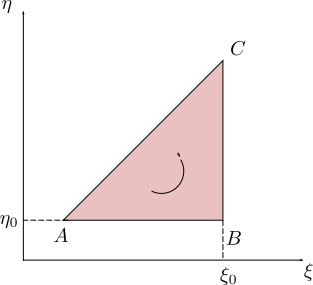
\includegraphics[width=0.2\textwidth]{figHyperRiman2.pdf}
\end{wrapfigure}
\begin{minipage}[t]{0.7\textwidth}
\[
	\oint\limits_{\partial D} \left(v \derp{w}{\eta}{} - w \derp{v}{\eta}{} \right) \, d\eta - \left(v \derp{w}{\xi}{} - w \derp{v}{\xi}{}\right)\, d\xi = 0\\
\]
\[
	\oint = \int\limits_A^B + \int\limits_B^C + \int\limits_C^A = 0
\]
\end{minipage}\\

\begin{multline*}
	\oint\limits_{\partial D}  \left(v \derp{w}{\eta}{} - w \derp{v}{\eta}{} \right) \, d\eta - \left(v \derp{w}{\xi}{} - w \derp{v}{\xi}{}\right)\, d\xi = \\ 
	= - \int\limits_A^B \left(v \derp{w}{\xi}{} - w \derp{v}{\xi}{} \right)\, d\xi + \int\limits_B^A \left(v \derp{w}{\eta}{} - w \derp{v}{\eta}{} \right)\, d\eta + \int\limits_C^A \left[\left(v \derp{w}{\eta}{} - w \derp{v}{\eta}{} \right)\, d\eta - \left(v \derp{w}{\xi}{} - w \derp{v}{\xi}{} \right)\, d\xi \right] = \\
	= - wv \Big|_A^B + 2 \int\limits_A^B w \derp{v}{\xi}{} d \xi + v w \Big|_B^C - 2 \int\limits_B^C w \derp{v}{\eta}{}\, d\eta + \int\limits_C^A [\ldots] = -2 w v\Big|_B + w v\Big|_A + w v\Big|_C + \int\limits_C^A [\ldots] = 0
\end{multline*}
\[
	w v\Big|_B = \frac{wv\Big|_A + w v\Big|_C}{2} + \frac{1}{2} \int\limits_C^A \left[ \left(v \derp{w}{\eta}{} - w \derp{v}{\eta}{} \right) - \left(v \derp{w}{\xi}{} - w \derp{v}{\xi}{} \right)\, d\xi\right]
\]
%($u_n$ -- производная по направлению нормали к кривой $S$), и выясним область, в которой решение определяется начальными условиями.


%Кривая $S$ задана уравнением
%\[
%	y = g(x)
%\]
%где $g(x)$ -- дифференциируемая функция. Наложим на кривую $S$ условие, чтобы всякая характеристика семейств $y - x = const$ и $y + x = const$ пересекала кривую $S$ не более одного раза (для этого нужно, чтобы $\abs{g'(x)} < 1$). 

%\begin{align*}
%	&v l[w] - w l^*[v] = v \left(\derps{v}{\xi}{\eta}+ \frac{1}{4} w\right) - w\left(\derps{v}{\xi}{\eta} + \frac{1}{4} v \right) = \frac{1}{2} \derp{}{\xi}{} \left(w \derp{w}{\eta}{} \right) - \frac{1}{2} \derp{}{\eta}{} \left(v \derp{v}{\xi}{} \right) \\
%	&v l[w] - w l^*[v] = \frac{1}{2} \frac{\partial}{\partial \xi}\left(v \der{w}{\eta}{} \right) - \frac{1}{2} \frac{\partial}{\partial \xi}\left(v \der{v}{\eta}{} \right) + \frac{1}{2} \frac{\partial}{\partial \eta}\left(v \der{w}{\eta}{} \right) - \frac{1}{2} \frac{\partial}{\partial \eta}\left(w \der{v}{\eta}{} \right)
%\end{align*}
%\[
%	\frac{1}{2} \frac{\partial}{\partial \xi}\left(v \der{w}{\eta}{} - w \der{v}{\eta}{} \right) + \frac{1}{2} \frac{\partial}{\partial \eta}\left( v \der{w}{\xi}{} - w \der{v}{\xi}{} \right) = 0
%\]
%Проинтегрируем это выражение
%\[
%	\iint\limits_D \frac{1}{2} \frac{\partial}{\partial \xi}\left(v \der{w}{\eta}{} - w \der{v}{\eta}{} \right) + \frac{1}{2} \frac{\partial}{\partial \eta}\left( v \der{w}{\xi}{} - w \der{v}{\xi}{} \right) d\xi d\eta = 0
%\]
%Применяем формулу Грина
%\[
%	\oint\limits_G \left(v \der{w}{\eta}{} - w \der{v}{\eta}{} \right) d\eta - \oint\limits_G \left(v \der{w}{\xi}{} - w \der{v}{\xi}{} \right) d\xi = 0
%\]
%\begin{multline*}
%	\oint = \int\limits_A^B + \int\limits_B^C+ \int\limits_C^A = \int\limits_A^B \left(v \der{w}{\eta}{} - w \der{v}{\eta}{} \right) d\eta - \int\limits_B^C \left(v \der{w}{\xi}{} - w \der{v}{\xi}{} \right) d\xi +\\{} + \oint\limits_G \left(v \der{w}{\eta}{} - w \der{v}{\eta}{} \right) d\eta -  \left(v \der{w}{\xi}{} - w \der{v}{\xi}{} \right) d\xi = 0
%\end{multline*}
%\[
%	- w v \Big|_A^B + \int\limits_A^B w \left(\der{v}{\xi}{} + \der{v}{\eta}{} \right) d \xi + v %w\Big|_B^C - \int\limits_B^C w \left(\der{v}{\eta}{} + \der{v}{\eta}{}\right) d \eta + \int\limits_C^A \ldots= 0
%\]
%%Потребуем чтобы выполнялись граничные условия:
%\begin{align*}
%	&AB: \der{v}{\xi}{} = 0\\
%	&BC: \der{v}{\eta}{} = 0\\
%\end{align*}
%\[
%	\frac{(wv)_A + (vw)_C}{2} + \frac{1}{2} \int\limits_C^A \left(v \der{w}{\eta}{} - w \der{v}{\eta}{} \right) d\eta -  \left(v \der{w}{\xi}{} - w \der{v}{\xi}{} \right) d\xi = (wv)_B
%\]

	
Найдём функцию Римана.
\[
	\derps{v}{\xi}{\eta} + \frac{1}{4} v = 0
\]
Будем искать $v$ в виде $v =\Phi(\lambda); \quad \lambda= \sqrt{(\xi - \xi_0)(\eta - \eta_0))}$\\
\begin{align*}
	&\derp{v}{\xi}{} =\Phi'(\lambda) \derp{\lambda}{\xi}{}  &\derps{v}{\xi}{\eta} = \derp{}{\eta}{} \left(f'(\lambda) \derp{\lambda}{\xi}{}\right) =\Phi'' \derp{\lambda}{\xi}{} \derp{\lambda}{\eta}{}  +\Phi' \derps{\lambda}{\xi}{\eta}
\end{align*}
\[
	\derps{\lambda}{\xi}{\eta} = \frac{(\xi - \xi_0)}{2 \sqrt{(\xi - 'xi_0)(\eta - \eta_0)}} = \frac{1}{2} \sqrt{\frac{\xi - \xi_0}{\eta -\eta_0}} \derp{\lambda}{\xi}{} = \frac{1}{2} \sqrt{\frac{\eta - \eta_0}{\xi - \xi_0}}
\]
\[
	\derps{\lambda}{\xi}{\eta} = \frac{1}{4 \sqrt{(\xi - 'xi_0)(\eta - \eta_0)}} = \frac{1}{4 \lambda}
\]
\begin{equation}
	\Phi'' + \frac{\Phi'}{\lambda} + \Phi = 0
	\label{equ:equRimanBessel}
\end{equation}
Уравнение \eqref{equ:equRimanBessel} является уравнением Бесселя нулевого порядка.
\[
	\Phi = J_0(\lambda) = \sum\limits_{k = 0}^{\infty} \frac{\lambda^{2k}}{2 k!!}, \quad \Phi(0) = 1
\] 
Итак, искомая функция Римана $v = J_0 (\lambda)$\\
на прямой $AB$
\[
	\lambda = 0 \Rightarrow \derp{v}{\xi}{} = J_0'(\lambda) \derp{\lambda}{\xi}{} \Big|_{\eta=\eta_0} = 0
\]
на прямой $BC$ 
\[
	\derp{v}{\eta}{} = J_0'(\lambda) \derp{\lambda}{\eta}{}\Big|_{\xi = \xi_0} = 0
\]
В точке $B$ $v(b) = 1 = v(A) = v(c)$. Так как $\xi = \eta \Rightarrow d\xi = d\eta$, тогда 
\[
	w(B) = \frac{w(A) + w(C)}{2} + \frac{1}{2} \int\limits_C^A \left[ v \left(\derp{w}{\eta}{} - \derp{w}{\xi}{} \right) - w \left(\derp{v}{\eta}{} - \derp{v}{\xi}{}\right)\right]\, d\xi
\]
Известно, что 
\[
	b\left(\derp{w}{\eta}{} - \derp{w}{\xi}{} \right) = - g\left(\frac{a}{b}\xi\right) - \frac{b_0}{a_0} f\left(\frac{a}{b} \xi\right)
\]
\begin{align*}
	&\derp{v}{\eta}{} = J_0'(\lambda) \frac{(\xi - \xi_0)}{\sqrt{(\xi - \xi_0)(\eta - \eta_0)}} & \derp{v}{\xi}{} = J'(\lambda) \frac{\eta - \eta_0}{\sqrt{(\eta - \eta_0)(\xi - \xi_0)}}
\end{align*}
\[
	\derp{v}{\eta}{} - \derp{v}{\xi}{} = J_0'(\lambda) \frac{(\eta_0 - \xi_0)}{\sqrt{(\eta - \eta_0) (\xi - \xi_0)}}
\]

В итоге получаем
\begin{multline}
	w (\xi_0, \eta_0) = \frac{f\left(\frac{a}{b} \eta_0 \right) + f\left(\frac{a}{b} \xi_0 \right)}{2} +{}\\
	+\frac{1}{2} \int\limits_{\xi_0}^{\eta_0} \left\{J_0(\lambda) \left(- \frac{1}{b}  \right) \left(g\left(\frac{a}{b}\xi\right) + \frac{b_0}{a_0} f\left(\frac{a}{b} \xi\right) \right) - f \left(\frac{a}{b} \xi \right) \frac{J'(\lambda)(\eta_0 - \xi_0)}{\sqrt{(\eta - \eta_0)(\xi - \xi_0)}} \right\} d\xi
\end{multline}
%\[
%	\xi  + \eta = 2 b t \quad t = \frac{\xi + \eta}{2 b} \quad x = \frac{(\xi +\eta)u}{2b}
%\]

%Найдём производные
%\[
%	\derps{v}{\xi}{\eta} = \frac{1}{4 \sqrt{(\xi - \xi_0)(\eta - \eta_0))}}
%\]
%\[
%	\der{v}{\xi}{} =\Phi'(\lambda) \der{\lambda}{\xi}{} 
%\]
%\[
%	\quad\Phi'' \frac{1}{4} +\Phi' \frac{1}{4 \sqrt{(\xi - \xi_0)(\eta - \eta_0))}} + \frac{1}{4} = 0
%\]

%Мы рассматривали похожее уравнение\\
%\[
%	y'' + \frac{1}{x}y' + y = 0
%\]
%функция Бесселя.
%\[
%\Phi = J_0(\lambda)
%\]
%\[
%	J_0(0) = 1
%\]

%В нашем случае искомая функция Римана - функция Бесселя. \\
%\[
%	v = J_0(\lambda)
%\]
%На прямой AB $\lambda = 0$. И мы получаем \\
%\[
%	AB: \der{v}{\xi}{} = J_0'(\lambda) \der{\lambda}{\xi}{}|_{\eta - \eta_0} = 0
%\]
%	
%Смотрим для точки B.\\
%\[
%	B: \xi = \xi_0 \eta = \eta_0 \rightarrow
%\]
%\begin{align*}
%	&\lambda = 0\\
%	&i_0(0) = 1\\
%	&v|_b J_0(0) = 1\\
%\end{align*}

%\includegraphics{graphic}

%\[
%	\derps{w}{\xi}{\eta} + \frac{1}{4} w = 0
%\]
%\[
%		\xi = \eta \quad w =\Phi(\frac{a}{b}\xi)
%\]
%\[
% b \left(\derp{w}{\xi}{} - \derp{w}{\eta}{}\right) = g\left(\frac{a}{b}\xi\right) + \frac{b_0}{a_0}\Phi\left(\frac{a}{b}\xi\right) 
%\]
%\begin{multline*}
%	w(\xi_0, \eta_0) = \frac{w_a + w_c}{2} + \frac{1}{2} \int\limits_c^a \left[\left(v\derp{w}{\eta}{} - w \derp{v}{\eta}{}\right)d\eta - \left(v\derp{w}{\xi}{} - w \derp{v}{\eta}{}\right)\, d\xi \right] = \\ = \frac{w_a - w_c}{2} + \frac{1}{2} \int\limits_c^a \left[v \left(\derp{w}{\eta}{} - \derp{w}{\xi}{}\right) - w \left(\derp{v}{\eta}{} - \derp{v}{\xi}{}\right)\right]d\xi
%\end{multline*}
%\[
%	v = J_0(\lambda): \quad \lambda = \sqrt{(\xi - \xi_0)(\eta - \eta_0)}
%\]
%\[
%	\xi = \frac{b}{a}(x + at)
%\]
%\[
%	\eta = \frac{b}{a}(x - at) \quad J_0(0) = 1
%\]
%\[
%	\derp{v}{\eta}{} = J_0'(\lambda) \frac{\xi - \xi_0}{\sqrt{(\xi - \xi_0)(\eta - \eta_0))}}
%\]
%\[
%	\derp{v}{\xi}{} = J'(\lambda) \frac{\eta - \eta_0}{\sqrt{(\xi - \xi_0)(\eta - \eta_0))}}
%\]
\end{example}

